%%%%%%%%%%%%%%%%%%%%%%%%%%%%%%%%%%%%%%%%%%%%%%%%%%%%%%%%%%%%%%%%%%%%%%%%%%%%%%%%
%%%%%%%%%%%%%%%%%%%%%%%%%%%%%%%%%%%%%%%%%%%%%%%%%%%%%%%%%%%%%%%%%%%%%%%%%%%%%%%%
\section{Ciclo da aprendizagem - PDCA}
\label{sec:cicloaprendizagem}
\index{Aprendizagem!PDCA}

\begin{wrapfigure}{r}{0.45\textwidth}
  \centering
%\smartdiagram[circular diagram:clockwise]{Fazer, Verificar, Atuar, Planejar}
    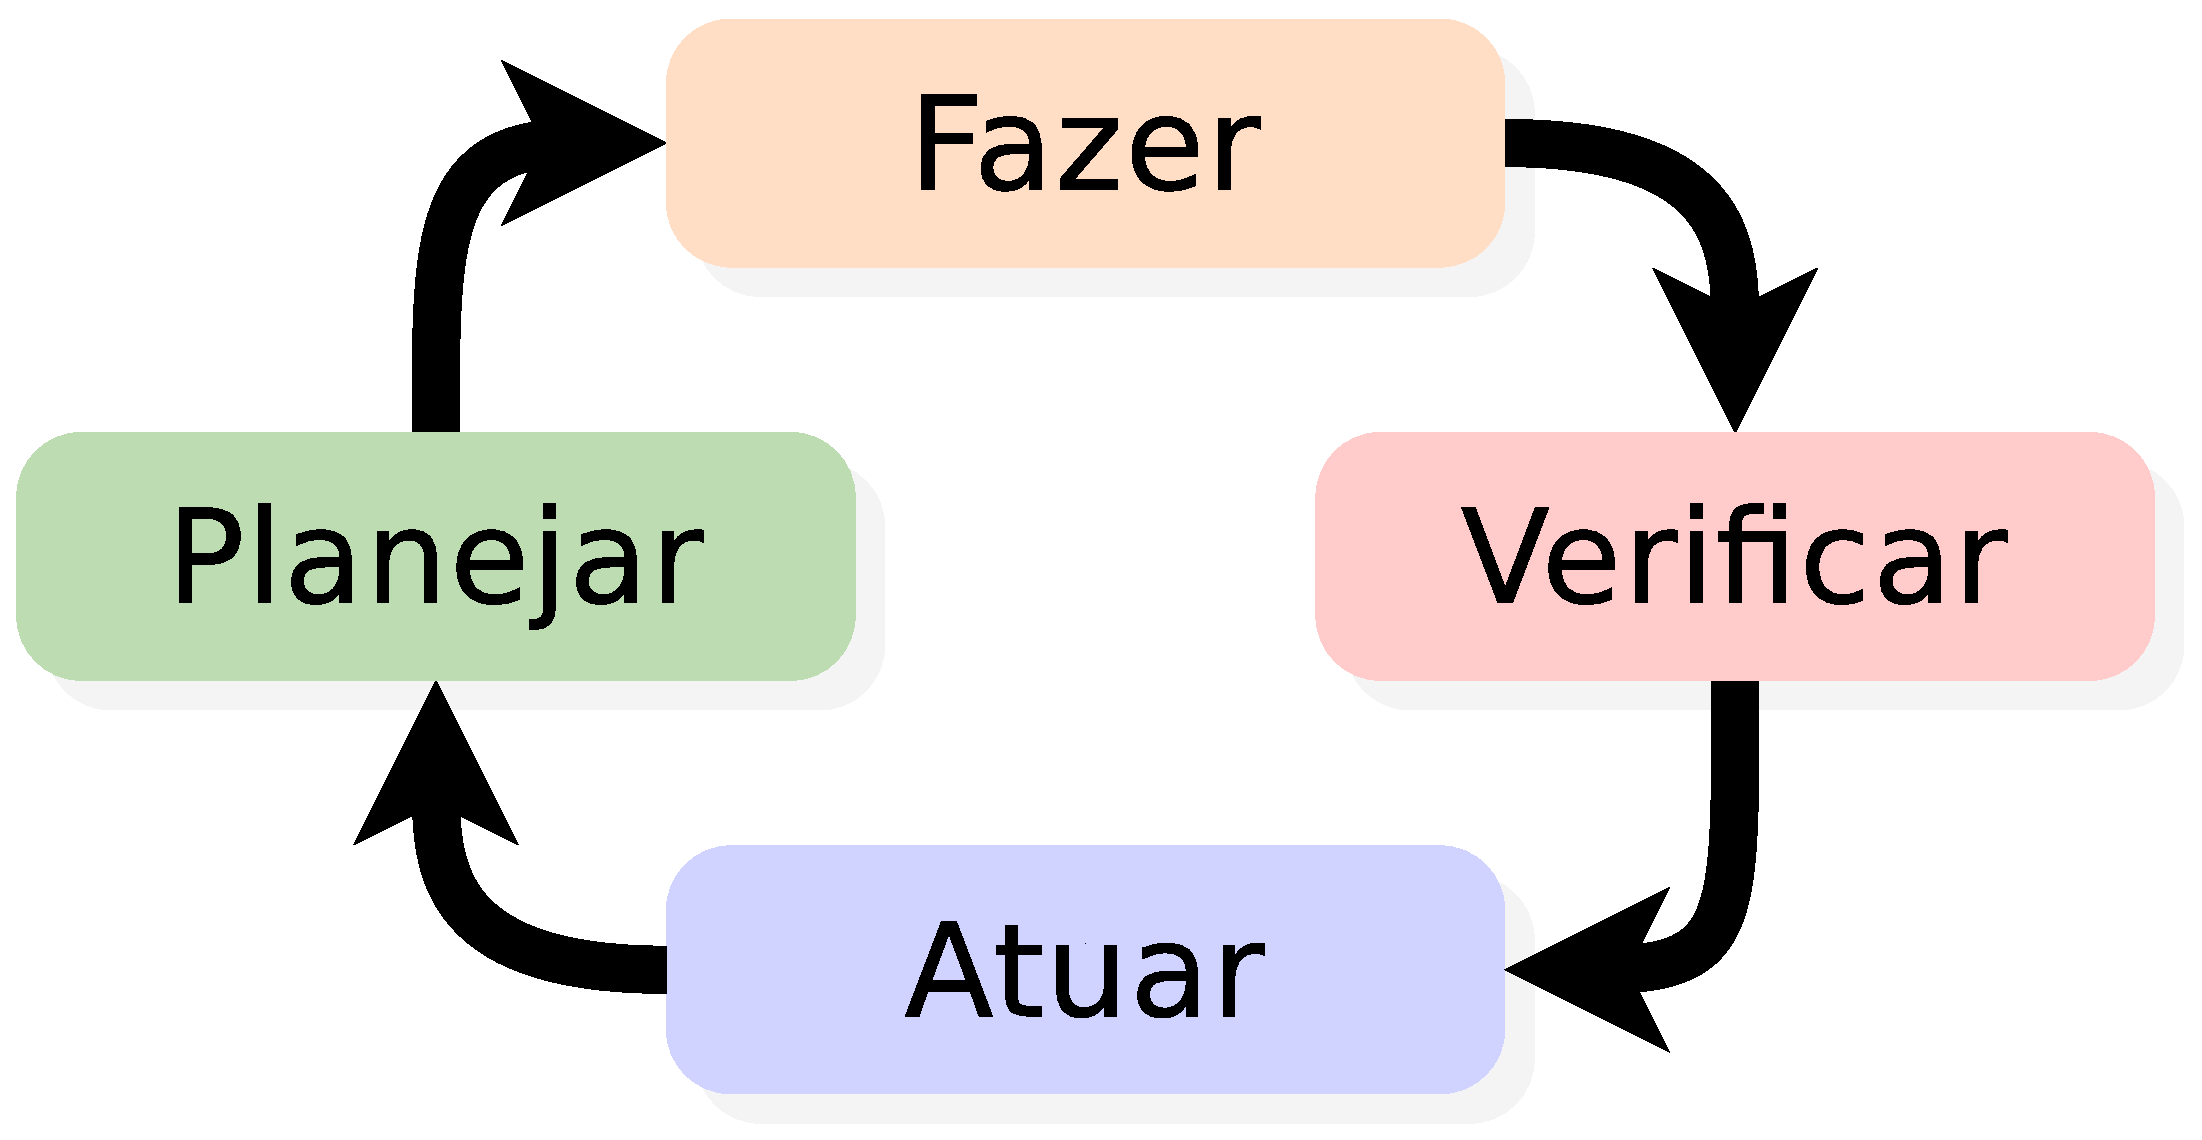
\includegraphics[width=0.42\textwidth]{chapters/cap-learning/ciclo2.eps}
\caption{Ciclo PDCA.}
\label{fig:ciclopdca}
\end{wrapfigure}
O ciclo que seguimos para potencializar nossa aprendizagem \cite[pp. 13]{mumford2001aprendendo},
em muitos aspectos se parece ao ciclo, para a melhoria continua, na gerencia de projetos 
\cite[pp. 4]{caloba2018gerenciamento} \cite[pp. 59]{teixeira2018gestao}.
Na literatura, este é conhecido como ``ciclo PDCA'';
a sigla vem das palavras em inglês: ``Plan'', ``Do'', ``Check'' e ``Act'';
estas podem ser interpretadas como: Planejar, fazer, verificar e atuar em consequência
\cite[pp. 59]{teixeira2018gestao} \cite[pp. 4]{caloba2018gerenciamento}.
Este fluxo de trabalho, também é chamado ``ciclo de Shewhart'' em honor a seu inventor,
ou ``ciclo de Demming'' em honor a um de seus grandes difusores no Japão
\cite[pp. 59]{teixeira2018gestao} \cite[pp. 4]{caloba2018gerenciamento}.
A Figura \ref{fig:ciclopdca} mostra em detalhe o fluxo de trabalho no ciclo PDCA.


\begin{description}
\item[Planejar:] Estabelecemos nosso objetivo no aprendizado; 
realizamos um planejamento do caminho que seguiremos para atingir nossos objetivos.
\item[Fazer, desenvolver:] Pomos em prática o trabalho anteriormente planejado;
coletamos dados sobre nosso desenvolvimento nas tarefas escolhidas.
\item[Verificar, conferir:] Comparamos o resultado obtido com o esperado;
realizamos uma avaliação de nosso despenho e competência.
\item[Atuar, agir, ajustar:] Tomamos ações corretivas no nosso plano de trabalho,
para diminuir as diferenças entre o resultado obtido e o esperado.
\end{description}
